\subsection{Calculating the Travel Interest Vector} 

We will evaluate the performance results of the
three CNNs used to classify the users' social media images. Naturally, the
speed and the accuracy of the program will be the deciding factor to form part
of the application.

\paragraph{Training results from the TensorFlow Keras sequential model}

We trained this model using the NVIDIA Tesla K80 GPU provided by Google Colab. At 16 epochs,
the model starts to overfit as the validation loss starts to increase, as shown
in figure~\ref{kerasresults}. This is why we chose to calculate the model's performance on the
testing set in the following subsections using the first 16 epochs. 

\begin{figure}[h]
\centering
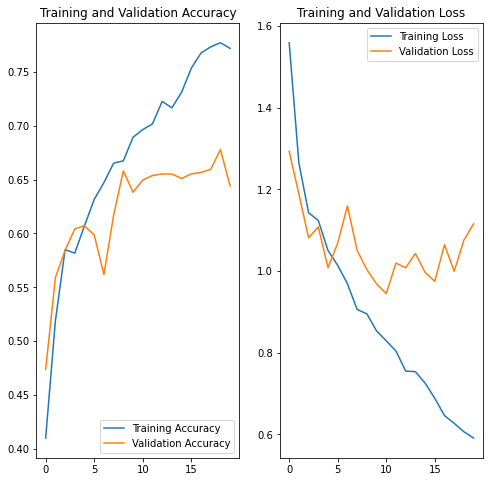
\includegraphics[width=0.5\textwidth]{Epoch_20.png}
\caption{Training and validation accuracy of the model on the testing and validation dataset}
\label{kerasresults}
\end{figure}

\paragraph{Performance comparison of the three models}

The following will evaluate the performance of the three CNNs used to classify
the user's photos. The model with the highest scores throughout all six
categories will be selected as the baseline for our application. 

The testing dataset consists of 500 images gathered using the Unsplash API. We
calculated the Accuracy, Precision, Recall and F1 Score on the testing set to
evaluate the models by extrapolating the number of true positive (TP), true
negative  (TN), false-negative (FN) and false positive (FP) label values as a
percentage over the dataset. 

The accuracy of the models, represented by:

\[Accuracy = (TP+TN) / (TP+FP+FN+TN)\]

The accuracy of the three models is shown in figure\ref{accuracy}. This shows
how resembling labels are to their `true' value. In this case, the Resnet 50,
Resnet 18, and Keras models have an average X, X, and X average accuracy,
respectively. The chart shows how, overall, the three models have very high
accuracy.

\begin{figure}[h]
\centering
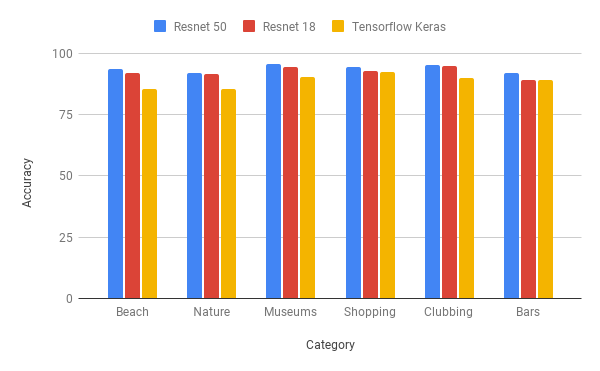
\includegraphics[width=0.7\textwidth]{Accuracy.png}
\caption{Accuracy of the Resnet-18, Resnet-50 and Tensorflow Keras Sequential}
\label{accuracy}
\end{figure}

The precision of the models, represented by

\[Precision = (TP) / (TP+FP)\]
The precision of the three models shown in figure~\ref{precision},
represents the ratio of correct predictions over the total positive labels.
In this case, the Resnet 50, Resnet 18, and Keras models have an average X, X,
and X precision rate, respectively. Again, the Resnet 50 has the best average
overall; however, the Keras model performed better for the 'clubbing' and
'bars' categories but very poorly in the shopping category.

\begin{figure}[h]
\centering
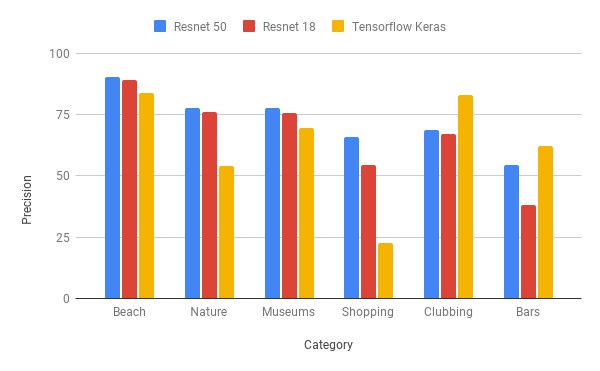
\includegraphics[width=0.7\textwidth]{Precision.png}
\caption{Precision of the Resnet-18, Resnet-50 and Tensorflow Keras Sequential}
\label{precision}
\end{figure}

The proportion of actual positive labels that the models identify correctly is
represented by the recall value calculated using 

\[Recall= (TP) / (TP+FN)\]

In this case, figure \ref{recall}
shows how for the clubbing and bar categories, although the Resnet models were
less accurate and less precise, they rarely labelled an image as a bar or a
club when they are not supposed to.

\begin{figure}[h]
\centering
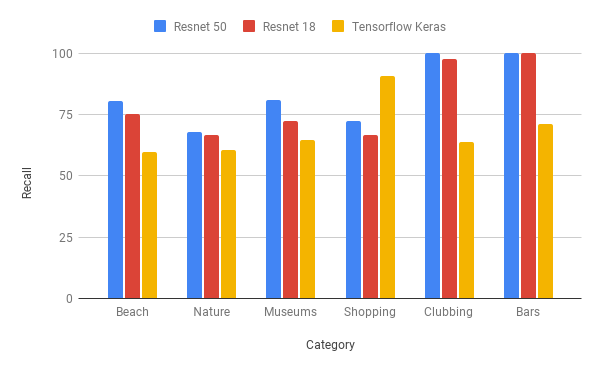
\includegraphics[width=0.7\textwidth]{Recall.png}
\caption{Recall of the Resnet-18, Resnet-50 and Tensorflow Keras Sequential}
\label{recall}
\end{figure}

The F1 score is the weighted average of Precision and Recall measured using:

\[F1 Score = 2*(Recall*Precision) / (Recall+Precision)\]
The Reset 50 has a pretty consistent and high score on
the testing dataset with an average F1 score of X, so
we decided to use it as our baseline for the tourist
itinerary generation application.

\begin{figure}[h]
\centering
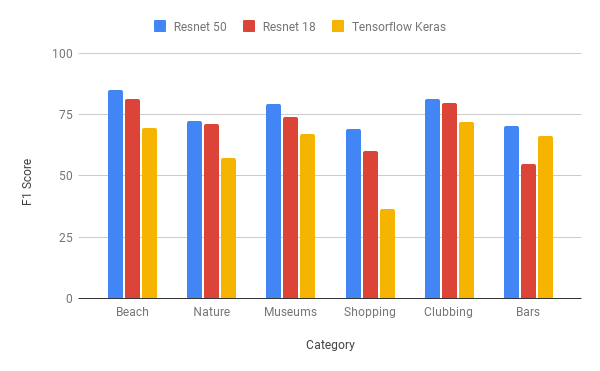
\includegraphics[width=0.7\textwidth]{F1Score.png}
\caption{F1 score of the Resnet-18, Resnet-50 and Tensorflow Keras Sequential}
\label{f1}
\end{figure}
